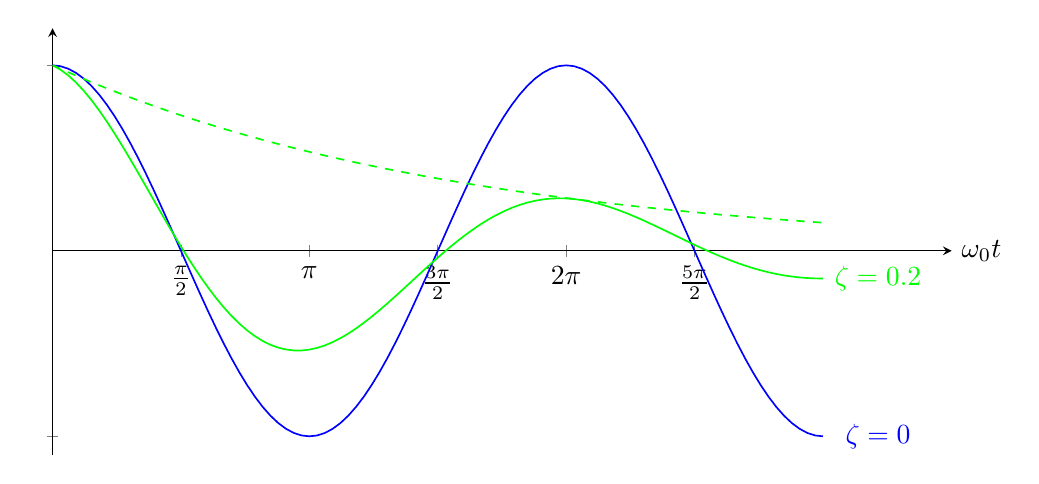
\begin{tikzpicture}
\begin{axis}[
    width=13cm, 
    height=7cm,
    axis x line=center, 
    axis y line=middle, 
    xlabel={$\omega_0 t$},
     x label style={at={(current axis.right of origin)}, right},
    samples=100,
    ymin=-1.1, ymax=1.2,
    xmin=0, xmax=11,
    domain=0:3*pi,
    xtick={ 1.5708, 3.14159, 4.7123889, 6.28318, 7.853981 },
    xticklabels={ 
    $\frac{\pi}{2}$, $\pi$, $\frac{3\pi}{2}$, $2\pi$, $\frac{5\pi}{2}$
    },
    ytick={-1,0,1},
    yticklabels={,,}
]
\addplot [mark=none, semithick, blue] {cos(deg(x))};
\addplot [mark=none, semithick, green, dashed] {exp(-0.2*x)};
\addplot [mark=none, semithick, green] {exp(-0.2*x)*cos(0.98*deg(x))};
\node[text=blue] at (axis cs:10.1,-1.0) {$\zeta=0$};
\node[text=green] at (axis cs:10.1,-0.15) {$\zeta=0.2$};
\end{axis}
\end{tikzpicture}
